%TCIDATA{Version=5.50.0.2960}
%TCIDATA{LaTeXparent=0,0,Master.tex}
                      
%TCIDATA{ChildDefaults=chapter:1,page:1}


\chapter{Introduction}

\label{chap:intro}

\begin{comment}
The two TeX boxes on the following line should only be used for the first
chapter
\end{comment}

%TCIMACRO{\TeXButton{pagenumbering}{\pagenumbering{arabic}}}%
%BeginExpansion
\pagenumbering{arabic}%
%EndExpansion
%TCIMACRO{\TeXButton{Start at page 0}{\addtocounter{page}{-1}}}%
%BeginExpansion
\addtocounter{page}{-1}%
%EndExpansion

\begin{quotation}
\LaTeX is a system for typesetting documents. Its first widely available
version, mysteriously numbered 2.09, appeared in 1985. \LaTeX{} is now
extremely popular in the scientific and academic communities, and it is used
extensively in industry. It has become a \emph{lingua franca} of the
scientific world; scientists send their papers electronically to colleagues
around the world in the form of \LaTeX{} input.\cite{Lamport-1994}
\end{quotation}

\section{Getting started}

This document serves three purposes.

\begin{itemize}
\item It contains some information on how to use \LaTeX~\cite{Lamport-1994}
and Scientific Word to typeset your thesis.

\item It serves as a template that you can use for your thesis. Make a copy.

\item It contains many examples and some advice.
\end{itemize}

By default, all text is double spaced, however, lengthy quotations and
footnotes must be singled spaced. The left margin is slightly wider than the
right margin. This is to compensate for binding.

See \url{http://www.mun.ca/sgs/go/guid_policies/guidelines_intro.php} for
the SGS\ guidelines.

\section{Some tips, pitfalls, and opinions}

\label{sec:hints}

\subsection{Text mode}

\begin{itemize}
\item Use the View menu to turn on all the following:\ Invisibles, Helper
lines, Helper Boxes, Markers, Status Bar. Use View\ \TEXTsymbol{>}%
\TEXTsymbol{>}\ Toolbars to ensure that most tool bars are displayed. (I\
use all except History and Exam). Rearrange the tool bars with the mouse
until you are happy.

\item In text mode, type ` twice to get a \textquotedblleft\ and type '
twice to get \textquotedblright .

\item In LaTeX a closing single quotation mark and an apostrophe are the
same character. Use the ' key.

\item When you need three `s or three 's in a row, you can use a
\textquotedblleft zero space\textquotedblright\ (see below) to clarify what
is what. For example:\ John said, \textquotedblleft I heard her yell
`Stop'{}\textquotedblright . There is a zero space between the ' and the
\textquotedblright .

\item In text mode, type - twice to get and en-dash --. Type - three times
to get an em-dash --- . (Use en-dashes only for ranges of numbers or years.
Use em-dashes for punctuation.)

\item In text mode, the - key gives a hyphen, not a minus sign. Compare $x-y$
to \textit{x-y}.

\item For various kinds of horizontal spaces Insert \TEXTsymbol{>}%
\TEXTsymbol{>}\ Spacing \TEXTsymbol{>}\TEXTsymbol{>}\ Horizontal space (or
Alt i s h). See table \ref{tab-spaces} for more shortcuts and descriptions.

%TCIMACRO{\TeXButton{B}{\begin{table}[tbp] \centering}}%
%BeginExpansion
\begin{table}[tbp] \centering%
%EndExpansion
%TCIMACRO{\TeXButton{B SingleSpaced}{\begin{singlespaced}}}%
%BeginExpansion
\begin{singlespaced}%
%EndExpansion
$%
\begin{tabular}{|l|l|l|p{5cm}|}
\hline\hline
\multicolumn{1}{||l|}{\textbf{Space}} &  & \textbf{Shortcut} & 
\multicolumn{1}{|p{5cm}||}{\textbf{Use}} \\ \hline\hline
Normal & a b & Space bar & Text mode \\ \hline
Required & etc.\ a & Shift-space\  & Text mode, after a ., !, or ? that does
not end a sentence \\ \hline
Nonbreaking & Table~\ref{tab-spaces} & Cntl-space & Text mode, where a line
break would be confusing. \\ \hline
Em-space & a\quad b &  & Math or text mode. \\ \hline
2 em-space & a\qquad b &  & Math or text mode. \\ \hline
Thin space & $x\,y$ & Cntl-, & In math mode only. \\ \hline
Thick space & $x\;y$ & Cntl-Shift-space & In math mode only. \\ \hline
Italic correction & \textit{f}\/; &  & If needed, between italic and roman
characters. \\ \hline
Zero space & '{}\textquotedblright &  & Between ' and \textquotedblright\ or
` and \textquotedblleft . \\ \hline
Negative thin & $\cap \!\!\!\bullet $ &  & Math only. (Best to avoid the
need.) \\ \hline
No indent &  &  & Before a paragraph that should not be indented. \\ \hline
Custom &  &  & When long or stretchy spaces are needed. \\ \hline
\end{tabular}%
$%
%TCIMACRO{\TeXButton{E SingleSpaced}{\end{singlespaced}}}%
%BeginExpansion
\end{singlespaced}%
%EndExpansion
\caption{Horizontal spaces}\label{tab-spaces}%
%TCIMACRO{\TeXButton{E}{\end{table}}}%
%BeginExpansion
\end{table}%
%EndExpansion

\item You can double click on a space to change its width and nature. I\
find it easier to select the space and hit Control-F5

\item Tip:\ You can change the properties of spaces, letters, tables, and
other objects by selecting the object and hitting Control-F5.

\item Pitfall:\ Speaking of spaces. LaTeX will insert a little an
extra-stretchy space between sentences. About 99\% of the time\ LaTeX has no
problem correctly identifying the end of a sentence. The rule is this:\ Any
period (.), exclamation point (!), or question mark (?) that does not follow
a capital letter and that is followed by a normal space marks the end of a
sentence. So:

\begin{itemize}
\item When a period (.), exclamation point (!), or question mark (?) does
not end a sentence, follow it with a \textquotedblleft nonbreaking
space\textquotedblright\ (Alt i s h b) or a \textquotedblleft required
space\textquotedblright\ (Alt i s h r). For example, if I\ wrote
\textquotedblleft Dr.~N. loves C%
%TCIMACRO{\TeXButton{@}{\@}}%
%BeginExpansion
\@%
%EndExpansion
.\textquotedblright , I'd put a nonbreaking space between \textquotedblleft
Dr.\textquotedblright\ and \textquotedblleft N\textquotedblright . I could
have put a required space between the \textquotedblleft
N.\textquotedblright\ and \textquotedblleft loves\textquotedblright , but
there is no need, as LaTeX will assume that this period does not end a
sentence. I\ chose a nonbreaking space between \textquotedblleft
Dr.\textquotedblright\ and \textquotedblleft N.\textquotedblright\ because I
didn't want a line-break between them. For long surnames, it may be
preferable to use a required space after an abbreviated title.

\item When a period (.), exclamation point (!), or question mark (?) does
end a sentence but also follows a capital letter, put a LaTeX \TEXTsymbol{%
\backslash}@ command between the letter and the punctuation mark. For
example in \textquotedblleft Dr.~N. loves C%
%TCIMACRO{\TeXButton{@}{\@}}%
%BeginExpansion
\@%
%EndExpansion
.\textquotedblright , I'd put a LaTeX \TEXTsymbol{\backslash}@ command
between the \textquotedblleft C\textquotedblright\ and the \textquotedblleft
.\textquotedblright . Alt i y t can be used to insert a TeX command.\ Then
put \TEXTsymbol{\backslash}@ in the text box and click OK.

\item A common error is to put a normal space rather than a required space
after \textquotedblleft i.e.\textquotedblright , \textquotedblleft
e.g.\textquotedblright , \textquotedblleft etc.\textquotedblright\ If they
don't end a sentence, follow it by a required, rather than a normal space.
For example:\ \textquotedblleft CDC, Univac, etc.\ are no more, i.e.\
defunct.\textquotedblright

\item When a period (.), exclamation point (!), or question mark (?) is
followed by a close parenthesis, LaTeX will treat the parenthesis as the end
of the sentence and the following space will be extra stretchy.

\item When a period (.), exclamation point (!), or question mark (?) is
followed by a single or double close quotation mark, LaTeX should treat the
quotation mark as the end of a sentence. However, thanks to an SW oddity,
this won't work with SW. At present I have no good workaround.

\item The following table illustrates how LaTeX deals with various cases:%
%TCIMACRO{\TeXButton{B SingleSpaced}{\begin{singlespaced}}}%
%BeginExpansion
\begin{singlespaced}%
%EndExpansion
\begin{equation*}
\begin{tabular}{|l|p{3.2cm}|}
\hline
Default behaviour & \textquotedblleft (M M m. M MMMM. \\ \hline
Required space & \textquotedblleft (M M m.\ M MMMM. \\ \hline
Paren after period & \textquotedblleft M M m.) M MMMM. \\ \hline
Quote after period. & (M M m.\textquotedblright\ M MMMM. \\ \hline
Period after capital. & \textquotedblleft (m M M. M MMMM. \\ \hline
\TEXTsymbol{\backslash}@ before period & \textquotedblleft (m M M%
%TCIMACRO{\TeXButton{@}{\@}}%
%BeginExpansion
\@%
%EndExpansion
. M MMMM. \\ \hline
\end{tabular}%
\end{equation*}%
%TCIMACRO{\TeXButton{E SingleSpaced}{\end{singlespaced}}}%
%BeginExpansion
\end{singlespaced}%
%EndExpansion
\end{itemize}

\item The `Noindent space' (Insert \TEXTsymbol{>}\TEXTsymbol{>}\ Spacing 
\TEXTsymbol{>}\TEXTsymbol{>}\ Horizontal Space... \TEXTsymbol{>}\TEXTsymbol{>%
}\ Noindent or Alt i s h n) is not really a space at all. It can be used at
the start of a paragraph to suppress its indentation. This is useful when a
list is used that is not at the end of a paragraph.

\item Usually TeX hyphenates without trouble. If it fails to hyphenate \emph{%
Entscheidungsproblem}, for example, correctly you can indicate all the
places where it can hyphenate such troublesome words, using Insert 
\TEXTsymbol{>}\TEXTsymbol{>}\ Spacing \TEXTsymbol{>}\TEXTsymbol{>}\ Break 
\TEXTsymbol{>}\TEXTsymbol{>}\ Discretionany Hyphen.

\item To indicate where line breaks are allowed insert an \textquotedblleft
allow break\textquotedblright\ command (Insert \TEXTsymbol{>}\TEXTsymbol{>}\
Spacing \TEXTsymbol{>}\TEXTsymbol{>}\ Break \TEXTsymbol{>}\TEXTsymbol{>}\
Allow break or Alt i s b a). For example, if I give a file name as
/usr/\allowbreak theo/\allowbreak docs/\allowbreak thesis/\allowbreak
Master.tex. I\ might do well to add an `allow break' after each / except the
first.

\item For URLs and URIs use, Insert \TEXTsymbol{>}\TEXTsymbol{>} TeX Object 
\TEXTsymbol{>}\TEXTsymbol{>} Tex Field ... and insert \texttt{\TEXTsymbol{%
\backslash}url\{\emph{your url}\}}. Follow the link %
\url{http://en.wikibooks.org/wiki/LaTeX/Hyperlinks} for more. This has
several advantages:\ It correctly typesets characters such as tildes. It
allows breaks at the right places. It sets the URL in typewriter font. It
will insert actual hyperlinks into the PDF copy of your thesis, if you
compile it with PDFLaTeX.
\end{itemize}

\subsection{Math mode}

\begin{itemize}
\item Control-m will switch to math mode. Control-t will switch to text mode.

\item I\ set up my User Setup (Tools \TEXTsymbol{>}\TEXTsymbol{>} User
setup) so that the spacebar after a space will switch from text mode to math
mode and a spacebar while in math mode will switch to text mode. That way,
two taps on the spacebar will switch modes and insert a space.

\item To get spaces in math mode, use Control-Shift-Spacebar to get a thick
space $f\;x$ and Control-Comma to get a thin space $f\,x$.

\item In math mode, the - key gives a minus sign, not a hyphen. Compare $x-y$
to \textit{x-y}.

\item In math-mode ' gives you a superscript prime. Compare \textit{x'} to $%
x^{\prime }$. If you really need an apostrophe, closing single quote, or
double quote, switch to text mode.

\item Control-d will insert a new math display as shown in (\ref{eqn:example}%
) 
\begin{equation}
\left( 
\begin{array}{c}
k \\ 
3%
\end{array}%
\right) +\frac{\left( 
\begin{array}{c}
k \\ 
2%
\end{array}%
\right) \left( 
\begin{array}{c}
k-2 \\ 
2%
\end{array}%
\right) }{2}=\frac{1}{(k-2)!}\ \sum_{i=0}^{k-3}(-1)^{i}\left( 
\begin{array}{c}
k-2 \\ 
i%
\end{array}%
\right) (k-2-i)^{k}\text{\quad .}  \label{eqn:example}
\end{equation}

\item When your cursor is at the end of the math display, the tab key will
toggle whether the display is numbered.

\item Opinion:\ Displays should be used when a formula might cause a bad
line break, when the formula is so tall that it will cause an irregular
distance between lines of text, or when it needs a number.

\item Opinion: It is good style to only number those displays that need to
be referred to in the text. I.e., that will be cross referenced.

\item Opinion:\ Usually it is best to \textbf{not} omit punctuation after
displayed math. I\ usually leave an em-space or a quad-space between the
math and the punctuation. For example:\ Now it is time to prove%
\begin{equation*}
P\sqsubseteq Q\text{\quad .}
\end{equation*}%
I make an exception\ for computer code. For example:\ 
\begin{equation*}
\text{\texttt{rm -r -f tmp}\quad .}
\end{equation*}%
If I put a period at the end of that sentence, it turns a command to delete
one directory into a command that also deletes the current directory. The
IEEE style guide suggests omitting the period at the end of sentence, but
not other punctuation.

\item Pitfall: After a display, be careful to only start a new paragraph if
you need one.

\item Pitfall: Multi-character identifiers should not be set in math mode's
default italic font, like this $\sin (first)$. Instead use the \textit{italic%
} font, like this $\sin (\mathit{first})$. The reason is that TeX uses
slightly different fonts for \textquotedblleft math
italic\textquotedblright\ and \textquotedblleft italic\textquotedblright .
The math italic font is designed so that the spacing between adjacent
letters is correct for implicit multiplication or function application $%
xy+fx $. The italic font is designed so the letter spacing is correct for
words. (I\ have set Shift-F6 to give \textit{italic font}.)

\item Opinion:\ I\ generally use italic (or math italic, if only one letter
is used)\ for variables and \textrm{an upright font such as Roman}
(Shift-F4) or \textsf{sans-serif} (Shift-F5) for constants, e.g. $\sin (x)$,
but $f(\mathrm{e})$. However, as Alan Perlis once said, \textquotedblleft
one man's constant is another man's variable\textquotedblright . If a
certain sequence of letters is intended to represent exactly the same thing
everywhere in your thesis, it's probably a constant. Otherwise, it is
probably a variable. (Aside:\ Strictly speaking, the opinion that constants
should be set upright should be applied to $e$, $i$, and $\pi $.\ However,
it is not easy to make an upright $\pi $ with Scientific Word, as the
required fonts are not included. The best I can do is $\mathrm{e}^{\mathrm{i}%
\pi }+1=0$.)

\item Use Control-( to enter a pair of round brackets\ (parenthesis) $\left(
x\right) $, Control-[ for square brackets $\left[ x\right] $, Control-\{ for
curly brackets (braces) $\left\{ x\right\} $, Control-\TEXTsymbol{<} for
angle brackets $\left\langle x\right\rangle $, Control-\TEXTsymbol{\backslash%
} for absolute values $\left\vert x\right\vert $, and Control-\TEXTsymbol{%
\vert} for norms $\left\Vert x\right\Vert $. Use Insert \TEXTsymbol{>}%
\TEXTsymbol{>}\ Brackets for any other combinations such as $\left\lceil
x\right\rfloor $.

\item Opinion:\ Bracket pairs entered this way will automatically enlarge.
Compare 
\begin{equation*}
\left( \frac{fx}{gx},hx\right) \text{ to }(\frac{fx}{gx},hx)
\end{equation*}%
The former is preferable.

\item However, avoid such \textquotedblleft paired
brackets\textquotedblright\ in in-line math (as opposed to displayed math).
The reason is that, LaTeX will not insert a line break between paired
brackets. If the brackets need to be enlarged, the formula, should likely
have been in a display anyway.

\item Opinion:\ Never use $\left[ {}\right] $ or $\left\{ {}\right\} $
brackets for simple grouping. E.g., $u\times \left( v+\left( w+\left(
xy\right) \right) \right) $ is preferable to $u\times \left\{ v+\left[
w+\left( xy\right) \right] \right\} $; the curly $\left\{ {}\right\} $
bracket should be used for sets and the square $\left[ {}\right] $ brackets
often have some meaning ascribed to them, for example, sequencing.

\item Never use less-than and greater-than signs in place of angle brackets.
Not only are they the wrong symbols, but LaTeX puts too much space or too
little space around them. Compare $P=<x^{\prime }=x>$ to $P=\left\langle
x^{\prime }=x\right\rangle $.

\item Invisible brackets (use Insert \TEXTsymbol{>}\TEXTsymbol{>}\ Brackets)
are useful sometimes. For example if I\ want to define a relation I\ might
use%
\begin{align*}
\left. f\equiv g\right. & \triangleq f\sqsubseteq g\wedge f\sqsubseteq g \\
f^{\smallsmile }& \triangleq \lambda s\lambda s^{\prime }\cdot f\,s^{\prime
}\,s
\end{align*}%
There are invisible brackets around $f\equiv g$ so that the vertical
alignment and the horizontal spacing is correct. Also use an invisible
bracket for cases:%
\begin{equation*}
f(x)=\left\{ 
\begin{array}{lll}
g(x) & \qquad & \text{if }x>0 \\ 
h(x) &  & \text{otherwise}%
\end{array}%
\right.
\end{equation*}

\item Use Control-$\downarrow $ and Control-$\uparrow $ for sub- and
superscripts $x_{i_{j}}^{2}$. Use the spacebar or $\rightarrow $ key to exit
the sub- or superscript.

\item Opinion: It is generally bad style to over use subscripts. If you ever
find you need two levels of sub(or super)scripts, rethink your notation.

\item Use markers (labels)\ and cross-references to refer numbered displays
(see (\ref{eqn:example}) on page \pageref{eqn:example}), sections (see
section \ref{sec:sections} on page \pageref{sec:sections}), figures and
tables. To enter a new marker\ (label) use the \textquotedblleft
Marker\textquotedblright\ button on the \textquotedblleft
Field\textquotedblright\ toolbar or Insert \TEXTsymbol{>}\TEXTsymbol{>}
Marker ... (Alt i e). To enter a cross-reference use \textquotedblleft Cross
Reference\textquotedblright\ button on the \textquotedblleft Typeset
object\textquotedblright\ toolbar or Insert\ \TEXTsymbol{>}\TEXTsymbol{>}\
Typeset Object \TEXTsymbol{>}\TEXTsymbol{>} Cross Reference ... (Alt i y r).
When you insert or edit a cross reference, markers in other chapters won't
show up in the list of markers; that's ok; just type in the marker.

\item Tip:\ Abbreviate frequently used symbols in math mode with automatic
substitutions (Tools \TEXTsymbol{>}\TEXTsymbol{>} Automatic Substitutions).
Develop your own system of substitutions that is easy for you to remember.
Unfortunately only letters can be used, so you can't start your
abbreviations with, say, a \TEXTsymbol{\backslash} . I\ use the letter q to
start many of my abbreviations. E.g. qa for $\wedge $, qo for $\vee $, qrb
for $\sqsubseteq $, and so on.

\item Table \ref{tab:keys} summarizes some of useful key combinations for
editing math. 
%TCIMACRO{\TeXButton{B}{\begin{table}[tbp] \centering}}%
%BeginExpansion
\begin{table}[tbp] \centering%
%EndExpansion
%TCIMACRO{\TeXButton{B SingleSpaced}{\begin{singlespaced}}}%
%BeginExpansion
\begin{singlespaced}%
%EndExpansion
\begin{tabular}{|l|l|}
\hline\hline
\multicolumn{1}{||l|}{\textbf{Key}} & \multicolumn{1}{|l||}{\textbf{Meaning}}
\\ \hline\hline
Control-m & Math mode \\ \hline
Control-t & Text mode \\ \hline
Control-d & Displayed math \\ \hline
Tab & Toggle display numbering \\ \hline
Tab & Go to next input box \\ \hline
Control-Shift-spacebar & Thick math space \\ \hline
Control-, & Thin math space \\ \hline
Control-g letter & Greek letter \\ \hline
Control-s letter & Symbol. E.g. Control-s v gives $\vee $ \\ \hline
Control-/ & Fraction $\frac{x}{y}$ \\ \hline
Control-(, Control-9 & $\left( x\right) $ \\ \hline
Control-[ & $\left[ x\right] $ \\ \hline
Control-\{ & $\left\{ x\right\} $ \\ \hline
Control-\TEXTsymbol{\backslash} & $\left\vert x\right\vert $ \\ \hline
Control-\TEXTsymbol{\vert} & $\left\Vert x\right\Vert $ \\ \hline
Control-\TEXTsymbol{<} & $\left\langle x\right\rangle $ \\ \hline
Control-$\downarrow $ & $x_{y}$ \\ \hline
Control-$\uparrow $ & $x^{y}$ \\ \hline
\end{tabular}%
%TCIMACRO{\TeXButton{E SingleSpaced}{\end{singlespaced}}}%
%BeginExpansion
\end{singlespaced}%
%EndExpansion
\caption{Some useful keys}\label{tab:keys}%
%TCIMACRO{\TeXButton{E}{\end{table}}}%
%BeginExpansion
\end{table}%
%EndExpansion
\end{itemize}

\subsection{Function keys}

Table \ref{tab:fkeys} on page \pageref{tab:fkeys} summarizes some useful
functions keys. You can reprogram most function keys with Tag \TEXTsymbol{>}%
\TEXTsymbol{>}\ Function Keys... Table \ref{tab:keys} on page \pageref%
{tab:keys} gives some other useful key combinations

%TCIMACRO{\TeXButton{B}{\begin{table}[tbp] \centering}}%
%BeginExpansion
\begin{table}[tbp] \centering%
%EndExpansion
%TCIMACRO{\TeXButton{B SingleSpaced}{\begin{singlespaced}}}%
%BeginExpansion
\begin{singlespaced}%
%EndExpansion
\begin{tabular}{|l|l|}
\hline\hline
\multicolumn{1}{||l|}{\textbf{Function Key}} & \multicolumn{1}{|l||}{\textbf{%
Meaning}} \\ \hline\hline
F1 & Help \\ \hline
F2 & Pop the top item tag \\ \hline
F3 & Body Text \\ \hline
F4 & Clear font \\ \hline
Shift-F4 & \textrm{Roman font} \\ \hline
F5 & \textbf{Bold} \\ \hline
Shift-F5 & \textsf{Sans-serif font} \\ \hline
Control-F5 & Edit Properties \\ \hline
F6 & \emph{Emphasis} \\ \hline
Shift-F6 & \textit{Italic font} \\ \hline
F7 & Numbered item \\ \hline
Shift-F7 & Indent code \\ \hline
F8 & Bullet item \\ \hline
Shift-F8 & Code \\ \hline
F9 & \texttt{Typewriter font} \\ \hline
Shift-F9 & $\mathcal{CALIGRAPHIC~FONT}$ \\ \hline
F10 & Access menu \\ \hline
F11 & Section \\ \hline
F12 & Subsection \\ \hline
Shift-F11 & Subsubsection \\ \hline
Shift-F12 & Sub$^{3}$section \\ \hline
\end{tabular}%
%TCIMACRO{\TeXButton{E SingleSpaced}{\end{singlespaced}}}%
%BeginExpansion
\end{singlespaced}%
%EndExpansion
\caption{Some useful function keys}\label{tab:fkeys}%
%TCIMACRO{\TeXButton{E}{\end{table}}}%
%BeginExpansion
\end{table}%
%EndExpansion

\section{Figures and Tables}

\subsection{Figures from image files}

Scientific Workplace has good support for figures if they come from an image
file. Use File \TEXTsymbol{>}\TEXTsymbol{>}\ Import Picture... or Alt-f-i 
%TCIMACRO{%
%\FRAME{ftbFU}{5.1747in}{3.3176in}{0pt}{\Qcb{A simplified view of LaTeX bibligraphy generation.}}{\Qlb{fig-bibtex}}{figure.png}{%
%\special{language "Scientific Word";type "GRAPHIC";maintain-aspect-ratio TRUE;display "USEDEF";valid_file "F";width 5.1747in;height 3.3176in;depth 0pt;original-width 4.9664in;original-height 3.1739in;cropleft "0";croptop "1";cropright "1";cropbottom "0";filename 'graphics/figure.png';file-properties "XNPEU";}}}%
%BeginExpansion
\ifcase\msipdfoutput
\FRAME{ftbFU}{5.1747in}{3.3176in}{0pt}{\Qcb{A simplified view of LaTeX
bibligraphy generation.}}{\Qlb{fig-bibtex}}{figure.png}{%
\special{language "Scientific Word";type "GRAPHIC";maintain-aspect-ratio
TRUE;display "USEDEF";valid_file "F";width 5.1747in;height 3.3176in;depth
0pt;original-width 4.9664in;original-height 3.1739in;cropleft "0";croptop
"1";cropright "1";cropbottom "0";filename
'graphics/figure.png';file-properties "XNPEU";}}%
\else
\begin{figure}[tb]\centering
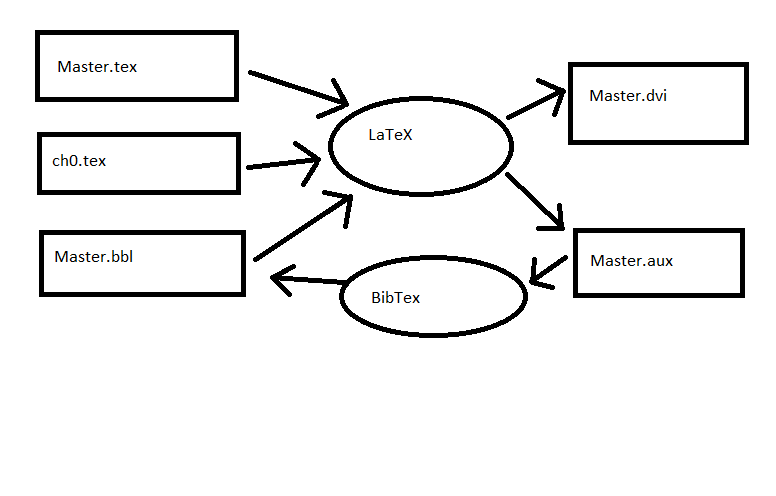
\includegraphics[
natheight=3.1739in, natwidth=4.9664in, height=3.3176in, width=5.1747in]
{C:/Users/theo/Documents/munthesis/graphics/figure__1.png}\caption{A
simplified view of LaTeX bibligraphy generation.}\label{fig-bibtex}%
\end{figure}%
\fi
%EndExpansion
For example see Figure \ref{fig-bibtex}. I suggest sticking to PNG or EPS
for image formats.

To make the figure float, pick \textquotedblleft floating\textquotedblright\
from the \textquotedblleft layout\textquotedblright\ tab of its properties.
Select \textquotedblleft top of page\textquotedblright\ and
\textquotedblleft bottom\ of page\textquotedblright .

\subsection{Other Figures}

Any LaTeX can be a figure. The trick is to use \textquotedblleft TeX
Fields\textquotedblright\ and use LaTeX's figure environment the way I did
to produce Figure \ref{fig-eqn-as-figure}

%TCIMACRO{\TeXButton{B Figure}{\begin{figure}[tb]}}%
%BeginExpansion
\begin{figure}[tb]%
%EndExpansion
\begin{equation*}
\begin{array}{lll}
AP & \sqsubseteq & AS \\ 
\downarrow I &  & \downarrow I \\ 
CP & \sqsubseteq & CS%
\end{array}%
\end{equation*}

%TCIMACRO{%
%\TeXButton{E Figure}{\caption{A commutativity diagram}\label{fig-eqn-as-figure}
%\end{figure}}}%
%BeginExpansion
\caption{A commutativity diagram}\label{fig-eqn-as-figure}
\end{figure}%
%EndExpansion

By the way there are several packages that make really fancy commutativity
diagrams. Figure \ref{fig-eqn-as-figure} simply uses a matrix (Insert 
\TEXTsymbol{>}\TEXTsymbol{>}\ Matrix --- which produces LaTeX's
\textquotedblleft array\textquotedblright\ environment) as a quick and dirty
way to make simple commutativity diagrams.

To create a figure that is not based on an image file, use the fragment
\textquotedblleft figure\textquotedblright\ or, for single spacing,
\textquotedblleft ssfigure\textquotedblright .\footnote{%
A fragment is a snippet of text that has been saved to a file. To insert a
fragment use the fragment \textquotedblleft drop down\textquotedblright\
list or type Alt-4. Then pick the fragment you need.
\par
You can create your own fragments, by selecting some text and then File 
\TEXTsymbol{>}\TEXTsymbol{>}\ Save Fragment ...}

\subsection{Tables}

Scientific Word has good support for tables, but not for the floating kind.
To make floating tables, you can use \textquotedblleft TeX
Fields\textquotedblright\ and LaTeX's \textquotedblleft
table\textquotedblright\ environment.

To make his easier, I've created a fragment \textquotedblleft
sstable\textquotedblright\ that inserts a single spaced table.

See Table \ref{tab:cusses} for an example.

%TCIMACRO{\TeXButton{B Table}{\begin{table}[tb]}}%
%BeginExpansion
\begin{table}[tb]%
%EndExpansion
%TCIMACRO{\TeXButton{B SingleSpaced}{\begin{singlespaced}}}%
%BeginExpansion
\begin{singlespaced}%
%EndExpansion

\begin{equation*}
\begin{tabular}{|l|r|}
\hline
\textbf{Language} & \textbf{Cusses} \\ \hline\hline
C\# & 20 \\ \hline
C++ & 56 \\ \hline
C & 28 \\ \hline
Java & 20 \\ \hline
JavaScript & 46 \\ \hline
Perl & 30 \\ \hline
PHP & 4 \\ \hline
Python & 10 \\ \hline
Ruby & 53 \\ \hline
\end{tabular}%
\end{equation*}%
%TCIMACRO{\TeXButton{E SingleSpaced}{\end{singlespaced}}}%
%BeginExpansion
\end{singlespaced}%
%EndExpansion
%TCIMACRO{%
%\TeXButton{Caption}{\caption{Cuss count by programming language.}}}%
%BeginExpansion
\caption{Cuss count by programming language.}%
%EndExpansion
\label{tab:cusses}%
%TCIMACRO{\TeXButton{E Table}{\end{table}}}%
%BeginExpansion
\end{table}%
%EndExpansion

\section{Bibliography and Citations}

Use BibTeX to create your bibliography (or references) section. \ It is well
worth reading Oren Patashnik's manual for BibTeX \cite{Patashnik-1988}.
While BibTeX files can be edited with any text editor, I prefer to use
JabRef. However using JabRef or a similar tool is no replacement for reading
the manual. BibTeX has a number of peculiarities that it pays to be aware
of. Be particularly careful of BibTeX entries you obtain from sources such
as the ACM; these often exhibit a low standard of care.

Citations are inserted using Insert \TEXTsymbol{>}\TEXTsymbol{>}\ Typeset
Object \TEXTsymbol{>}\TEXTsymbol{>}\ Citation.

My favourite citation style is `Harvard style' or (\textquotedblleft
named\textquotedblright\ style) with square brackets. It looks like this

\begin{quotation}
LaTeX was created by Lamport \cite{Lamport-1994}.
\end{quotation}

If you don't like the way the author's name is sometimes repeated, as it is
in the preceding example, you can use the \texttt{\TEXTsymbol{\backslash}%
shortcite}, which shows only the year in brackets. You can enter such a
command as a \textquotedblleft TeX Field\textquotedblright\ (Menu Insert 
\TEXTsymbol{>}\TEXTsymbol{>}\ Typeset\ Object \TEXTsymbol{>}\TEXTsymbol{>}\
TeX Field). Or use the \textquotedblleft shortcite\textquotedblright\
fragment.

\begin{quotation}
LaTeX was created by Lamport 
%TCIMACRO{\TeXButton{Short Cite}{\shortcite{Lamport-1994}}}%
%BeginExpansion
\shortcite{Lamport-1994}%
%EndExpansion
.
\end{quotation}

\noindent This removes the temptation to do this sort of thing

\begin{quotation}
LaTeX was created by \cite{Lamport-1994}.
\end{quotation}

\noindent Which you should not do. (It suggests that LaTeX was created by a
book, which it was not.)\ Your sentences should read correctly with all
citations removed.

Many electrical and computer engineers use IEEE style, which is shorter, but
harder on the reader. It looks like this

\begin{quotation}
LaTeX was created by Lamport [1].
\end{quotation}

\noindent Some supervisors may insist on IEEE style. To get IEEE style
citations (and bibliography), double click on the BIBTEX field in the master
file and select an IEEE style. Then remove named.cite from the
\textquotedblleft Package Options\textquotedblright\ list for the master
document (Typeset \TEXTsymbol{>}\TEXTsymbol{>}\ Options and Packages 
\TEXTsymbol{>}\TEXTsymbol{>}\ Package Options).
